\documentclass[conference,10pt]{IEEEtran}
\usepackage{amsmath}
\usepackage{fontspec}
\setmainfont{STIX Two Text}
\usepackage{unicode-math}
\setmathfont{STIX Two Math}
\usepackage{array,graphicx,booktabs,siunitx,multirow,microtype,xcolor}
\usepackage{tikz}
\usetikzlibrary{arrows.meta,positioning,fit,calc}
\usepackage[hidelinks]{hyperref}
\sisetup{group-separator={,},group-minimum-digits=4}
\newcommand{\MHs}{\,MH/s}

\begin{document}

\title{Supercomputing, Built from Lab Desktops:\\Design and Controlled Evaluation of\\a Four-Node Commodity Cluster}

\author{\IEEEauthorblockN{Divyansh Shukla, Abhinav Dhoke, Sneha Kumari, Vanshika Wadhwa, and Ankush Kumar}
\IEEEauthorblockA{Cluster Kit project\\
\href{https://github.com/TheDivyanshShukla/cluster-kit}{github.com/TheDivyanshShukla/cluster-kit}}}

\maketitle

\begin{abstract}
Small clusters assembled from ordinary desktop computers can give students and small laboratories access to parallel computing without dedicated high-performance hardware. This paper presents Cluster Kit, a lightweight master--worker framework that applies the principles of cluster supercomputers at classroom scale. Nodes find each other automatically by UDP broadcast, and work is distributed over persistent TCP connections with pull-based self-scheduling and two-deep chunk pipelining, so no host lists, remote shells or per-node configuration are needed. We evaluate it it on four identical Ubuntu workstations (12 hardware threads each) connected by a wired LAN. The workload is a SHA-256 partial-preimage search. Each configuration (every node alone, and 2, 3 and 4 nodes) was repeated seven times in an interleaved order, and comparisons use exact permutation tests and bootstrap confidence intervals. Four nodes sustained a median throughput of \SI{87.38}{\MHs}, a speed-up of 3.86 (95\% CI 3.81--3.89) over the mean single node and a parallel efficiency of 96.4\% relative to the sum of the nodes' individual rates. Every added node increased throughput significantly ($p = 0.0003$, the minimum attainable with seven repeats). The Karp--Flatt experimentally determined serial fraction stayed between 0.4\% and 1.3\%. Work was shared evenly (23.9--25.7\% per node) without static partitioning. We also show that an earlier informal comparison reporting a 17-fold gain was confounded, and we discuss threats to validity.
\end{abstract}

\begin{IEEEkeywords}
cluster computing, parallel efficiency, speed-up, self-scheduling, service discovery, UDP broadcast, MPI, SHA-256
\end{IEEEkeywords}

\section{Introduction}
High-performance computing (HPC) has traditionally relied on purpose-built machines, but since the Beowulf project~\cite{beowulf} it has been understood that commodity computers on a commodity network can form a useful parallel machine. University laboratories contain many such computers that sit idle for much of the day. A framework that turns them into a temporary cluster with minimal set-up has teaching value, because it makes concepts such as speed-up, efficiency and load balancing measurable, and practical value for workloads that split into independent tasks.

Performance claims about such systems are often based on single runs, mismatched hardware or different software on each side of a comparison, which makes them hard to interpret~\cite{hoefler}. An earlier informal measurement of the system studied here had exactly this problem (Section~\ref{sec:informal}).

This paper makes three contributions:
\begin{enumerate}
\item It describes the design of \emph{Cluster Kit}, a master--worker engine written in Rust that uses pull-based self-scheduling and pipelined chunk delivery over a minimal binary TCP protocol (Section~\ref{sec:design}).
\item It reports a controlled scaling experiment on four identical nodes, with repeated, interleaved measurements, confidence intervals and hypothesis tests (Sections~\ref{sec:method}--\ref{sec:results}).
\item It analyses the results with the Karp--Flatt metric, identifies a performance anomaly on the head node, and corrects an earlier confounded comparison (Section~\ref{sec:discussion}).
\end{enumerate}

\section{Background and Related Work}\label{sec:background}
\subsection{Scaling laws}
For $p$ processors, the speed-up is $S_p = T_1/T_p$ and the parallel efficiency is $E_p = S_p/p$. Amdahl's law~\cite{amdahl} bounds the speed-up of a fixed-size problem with serial fraction $f$ by $S_p \le 1/(f + (1-f)/p)$. Gustafson~\cite{gustafson} observed that in practice the problem size grows with the machine, so the \emph{scaled} speed-up of a fixed-time workload is $S_p = p - f(p-1)$. Karp and Flatt~\cite{karpflatt} proposed estimating the serial fraction from measurements,
\begin{equation}
e_p = \frac{1/S_p - 1/p}{1 - 1/p},
\label{eq:kf}
\end{equation}
where a constant $e_p$ indicates an inherently serial component and a growing $e_p$ indicates overhead that increases with $p$.

\subsection{Distribution frameworks}
MPI~\cite{mpi} is the standard for tightly coupled HPC applications but requires an identical software environment and launcher on every node. MapReduce~\cite{mapreduce} and Dask~\cite{dask} provide higher-level task models with richer scheduling and data movement at the cost of larger runtimes. Volunteer-computing systems such as BOINC~\cite{boinc} distribute independent work units to untrusted machines over the Internet. Cluster Kit sits at the opposite end: a single small binary for a trusted LAN, intended for workloads that split into independent ranges.

\subsection{Self-scheduling}
When tasks are assigned statically, the slowest node determines the completion time. Self-scheduling lets each worker request work when idle; chunk size trades scheduling overhead against load imbalance at the end of the job~\cite{factoring}.

\subsection{Workload}
SHA-256~\cite{fips180} maps any input to a 256-bit digest that is, for practical purposes, uniformly distributed. Finding an input whose digest begins with $k$ zero hexadecimal digits therefore needs $16^k$ attempts on average and cannot be done faster than by trying inputs. This is the structure of proof-of-work in Bitcoin~\cite{bitcoin}, and it makes a clean benchmark: tasks are independent, inputs and outputs are tiny, and the expected number of matches is known in advance.

\section{System Design}\label{sec:design}

\begin{figure*}[t]
\centering
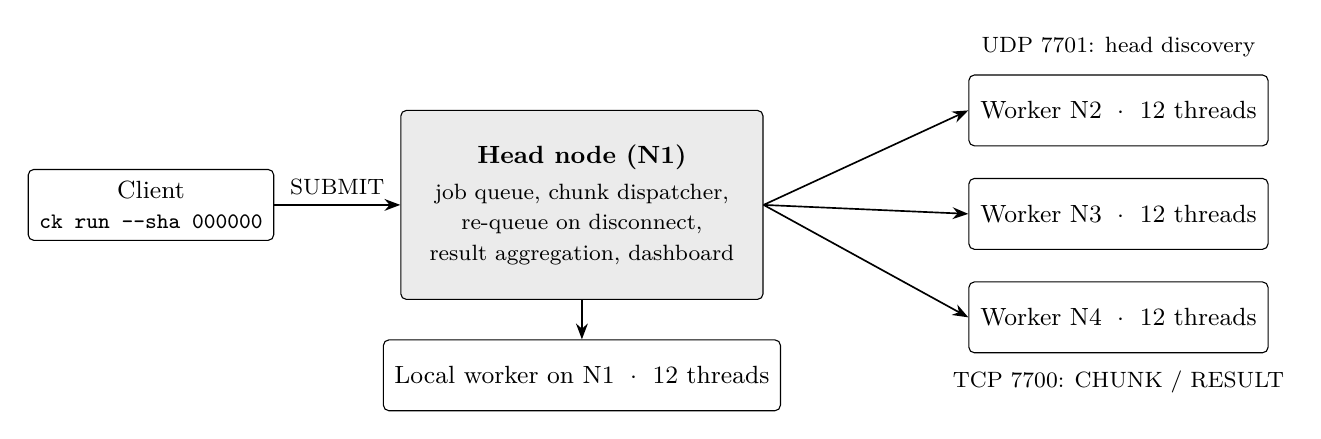
\begin{tikzpicture}[
  node distance=6mm and 14mm, font=\small,
  box/.style={draw, rounded corners=2pt, minimum height=9mm, align=center, inner sep=4pt},
  head/.style={box, fill=black!8, minimum width=46mm, minimum height=24mm},
  arr/.style={-{Stealth[length=2mm]}, semithick}]
  \node[box, minimum width=28mm] (client) {Client\\\footnotesize\texttt{ck run --sha 000000}};
  \node[head, right=16mm of client] (head) {\textbf{Head node (N1)}\\[2pt]\footnotesize job queue, chunk dispatcher,\\\footnotesize re-queue on disconnect,\\\footnotesize result aggregation, dashboard};
  \node[box, right=26mm of head, yshift=12mm, minimum width=38mm] (w2) {Worker N2 \;$\cdot$\; 12 threads};
  \node[box, below=4mm of w2, minimum width=38mm] (w3) {Worker N3 \;$\cdot$\; 12 threads};
  \node[box, below=4mm of w3, minimum width=38mm] (w4) {Worker N4 \;$\cdot$\; 12 threads};
  \node[box, below=5mm of head, minimum width=46mm] (local) {Local worker on N1 \;$\cdot$\; 12 threads};
  \draw[arr] (client) -- node[above, font=\footnotesize]{SUBMIT} (head);
  \draw[arr] (head.east) -- (w2.west); \draw[arr] (head.east) -- (w3.west); \draw[arr] (head.east) -- (w4.west);
  \draw[arr] (head) -- (local);
  \node[font=\footnotesize, align=center, below=1mm of w4] {TCP 7700: CHUNK / RESULT};
  \node[font=\footnotesize, align=center, above=1mm of w2] {UDP 7701: head discovery};
\end{tikzpicture}
\caption{Cluster Kit architecture. Workers discover the head by UDP broadcast and keep one persistent TCP connection. Each worker holds up to two chunks (one computing, one queued); every RESULT message also requests the next chunk. The head node additionally runs a local worker.}
\label{fig:arch}
\end{figure*}

Cluster Kit (Fig.~\ref{fig:arch}) consists of a single executable, \texttt{ck}, that runs in one of three roles.

\textbf{Head.} The head accepts a job, defined as an integer range $[a, b)$, a chunk size and a task, and dispatches chunks on request. It records which chunks each worker holds, so that if a worker disconnects its unfinished chunks are re-queued for others. It aggregates results and serves a live dashboard over HTTP. By default the head also starts a local worker, so a one-node cluster is a valid configuration.

\textbf{Discovery (UDP).} The head periodically broadcasts a small UDP beacon on port 7701. A worker started anywhere on the same subnet listens for the beacon, learns the head's address and connects; an explicit address can be given when broadcasts are blocked. UDP suits this role because a broadcast reaches every machine on the subnet in a single datagram and needs no prior knowledge of addresses, and a lost beacon is harmless since the next one follows shortly. Nodes can therefore join or leave a running cluster without editing any host list.

\textbf{Transport (TCP).} Chunks and results, by contrast, must not be lost or reordered, so each worker keeps one persistent TCP connection to the head on port 7700. Keeping the connection open avoids a handshake per chunk.

\textbf{Workers.} After connecting, a worker requests work. Each chunk is divided among all hardware threads using the Rust \emph{rayon} data-parallel library~\cite{rayon}. The worker keeps a pipeline of two chunks: while one is being computed, the next has already arrived, which hides network latency. A returned RESULT also serves as the request for the next chunk, so faster nodes automatically receive more work (self-scheduling).

\textbf{Protocol.} Messages use a fixed frame of one byte for the message type, a 32-bit little-endian length and a binary payload. A RESULT carries the job and range identifiers, the result body and the compute time the worker spent on the chunk, which the head uses for the per-node statistics in Section~\ref{sec:pernode}.

\textbf{Tasks.} Besides the built-in SHA-256 search used here, a job can run an arbitrary program on each sub-range, or the head can send a script to workers that do not have it. The repository also contains a Python/Dask engine and a distributed video-analytics system; neither is evaluated in this paper.

\section{Methodology}\label{sec:method}

\subsection{Testbed}
Table~\ref{tab:testbed} summarises the hardware and Fig.~\ref{fig:testbed} shows the physical set-up. All four nodes are the same model and ran the same operating system and the same \texttt{ck} binary, built once on N1 and copied to the other nodes.

\begin{figure}[t]
\centering
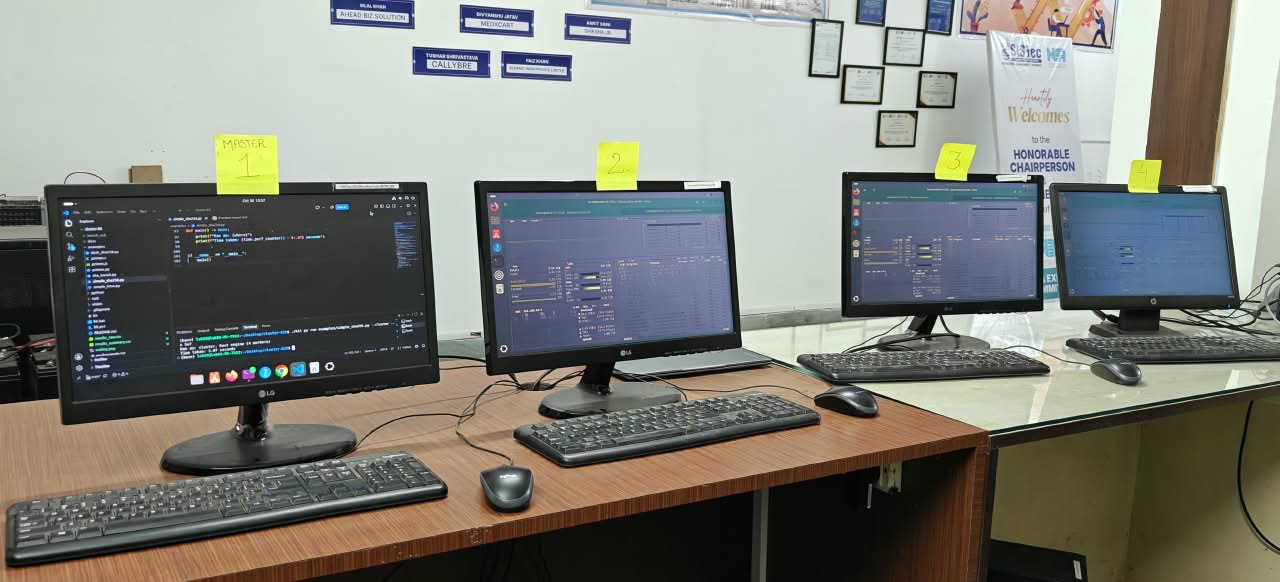
\includegraphics[width=\columnwidth]{img/testbed.jpg}
\caption{The testbed: four identical lab desktops on one wired LAN. The node labelled ``Master 1'' (N1) is the head; nodes 2--4 are workers.}
\label{fig:testbed}
\end{figure}

\begin{table}[t]
\caption{Experimental testbed}
\label{tab:testbed}
\centering
\begin{tabular}{@{}ll@{}}
\toprule
Nodes & 4 identical desktops (mainboard MS-7D22) \\
Per node & 12 hardware threads, 7.1\,GiB RAM \\
OS & Ubuntu 26.04.1 LTS, Linux 7.0 \\
Network & wired Ethernet LAN, RTT $<1$\,ms \\
Roles & N1 (192.168.10.122): head + worker \\
 & N2 (.200), N3 (.3), N4 (.5): workers \\
Engine & \texttt{ck} (Rust), CPU only \\
\bottomrule
\end{tabular}
\end{table}

\subsection{Workload and configurations}
Each run hashes the integers $1,\dots,n$ with SHA-256 and counts digests that start with \texttt{000000} (probability $16^{-6}$ per hash). Seven configurations were measured: each node alone (N1--N4), and clusters of $p = 2, 3, 4$ nodes, built by adding N2, N3 and N4 to N1 in that order. The range size $n$ was chosen per configuration so that a run lasts about \SI{3}{s} (Table~\ref{tab:configs}); the work per node is therefore approximately constant, which is the fixed-time (scaled) regime of Gustafson~\cite{gustafson}.

\subsection{Protocol}
After one warm-up run, the seven configurations were run seven times each in round-robin order, so that slow drifts such as heat or background activity affect all configurations similarly instead of being confounded with one of them~\cite{hoefler}. Throughput is $X = n/t$, where $t$ is the wall-clock time from job submission to the last result, as measured by the client.

\subsection{Metrics}
Because N1 turned out to be slower than the other nodes (Section~\ref{sec:anomaly}), a speed-up relative to N1 alone would overstate the benefit of clustering. We therefore report three measures:
\begin{align}
S_p &= X_p / \bar{X}_1, \qquad \bar{X}_1 = \tfrac{1}{4}\textstyle\sum_{i=1}^{4} X^{(i)}_1, \\
E_p &= X_p \Big/ \textstyle\sum_{i \in \mathcal{N}_p} X^{(i)}_1, \label{eq:eff}
\end{align}
where $X^{(i)}_1$ is the median rate of node $i$ alone and $\mathcal{N}_p$ is the set of nodes used. Equation~\eqref{eq:eff} accounts for heterogeneous node speeds: $E_p = 1$ means the cluster is exactly as fast as its members working separately. For comparison we also give the speed-up relative to N1. The serial fraction $e_p$ is computed from $S_p$ with~\eqref{eq:kf}.

\subsection{Statistics}
Medians are used as point estimates. Confidence intervals for means use the $t$ distribution. Confidence intervals for speed-ups are percentile bootstrap intervals with 5{,}000 resamples~\cite{bootstrap}. Differences between configurations are tested with one-sided exact permutation tests on the seven repeat throughputs of each~\cite{permutation}. With $7+7$ observations there are $\binom{14}{7} = 3{,}432$ splits, so the smallest attainable $p$-value is $1/3{,}432 \approx 0.0003$.

\section{Results}\label{sec:results}

\begin{table*}[t]
\caption{Throughput of all configurations (seven repeats each). MH/s = $10^6$ hashes per second. CV = coefficient of variation.}
\label{tab:configs}
\centering
\begin{tabular}{@{}lrrrrrrr@{}}
\toprule
Configuration & Nodes & Threads & $n$ per run & Median (MH/s) & Mean $\pm$ 95\% CI (MH/s) & CV (\%) & Matches \\
\midrule
N1 (head) & 1 & 12 & \num{68000000} & 20.55 & 20.92 $\pm$ 0.93 & 4.78 & 5 \\
N2 & 1 & 12 & \num{70000000} & 23.38 & 23.32 $\pm$ 0.17 & 0.78 & 5 \\
N3 & 1 & 12 & \num{70000000} & 23.37 & 23.35 $\pm$ 0.14 & 0.67 & 5 \\
N4 & 1 & 12 & \num{70000000} & 23.35 & 23.34 $\pm$ 0.04 & 0.20 & 5 \\
\midrule
$p=2$ (N1--N2) & 2 & 24 & \num{130000000} & 44.86 & 44.69 $\pm$ 1.16 & 2.80 & 8 \\
$p=3$ (N1--N3) & 3 & 36 & \num{200000000} & 67.48 & 67.20 $\pm$ 1.50 & 2.40 & 16 \\
$p=4$ (N1--N4) & 4 & 48 & \num{270000000} & 87.38 & 87.85 $\pm$ 1.15 & 1.42 & 21 \\
\bottomrule
\end{tabular}
\end{table*}

\subsection{Throughput scaling}
Table~\ref{tab:configs} lists all configurations and Fig.~\ref{fig:throughput} shows throughput against the number of nodes. Throughput rose from \SI{20.55}{\MHs} on N1 alone to \SI{87.38}{\MHs} on four nodes, closely following the ideal line given by the sum of the participating nodes' individual rates.

\begin{figure}[t]
\centering
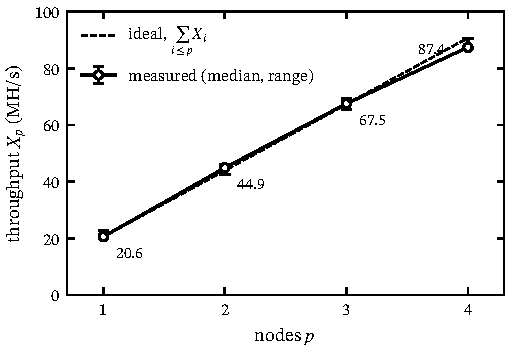
\includegraphics[width=\columnwidth]{fig_throughput.pdf}
\caption{Median throughput versus number of nodes; bars show the range of the seven repeats. The dashed line is the sum of the participating nodes' individual rates.}
\label{fig:throughput}
\end{figure}

\subsection{Speed-up, efficiency and serial fraction}
Table~\ref{tab:scaling} and Fig.~\ref{fig:speedup} give the derived metrics. Relative to the mean single node, four nodes are 3.86 times faster (95\% CI 3.81--3.89), an efficiency of 96.4\%. For $p = 2$ and $3$ the efficiency is slightly above 100\%; the excess (0.3--2.1\%) is within the run-to-run variation of the single-node baselines and is not evidence of super-linear behaviour. The Karp--Flatt serial fraction stays between 0.004 and 0.013 and does not grow steadily with $p$, so there is no sign of overhead increasing quickly with cluster size over this range.

\begin{table}[t]
\caption{Scaling metrics (medians). $S_p$ is relative to the mean single node $\bar{X}_1 = 22.66$\,MH/s.}
\label{tab:scaling}
\centering
\setlength{\tabcolsep}{4pt}
\begin{tabular}{@{}crrcrr@{}}
\toprule
$p$ & $X_p$ & $S_p$ [95\% CI] & vs N1 & $E_p$ (\%) & $e_p$ \\
\midrule
1 & 20.55 & 0.91 [0.89, 0.95] & 1.00 & 100.0 & -- \\
2 & 44.86 & 1.98 [1.92, 2.03] & 2.18 & 102.1 & 0.010 \\
3 & 67.48 & 2.98 [2.87, 3.05] & 3.28 & 100.3 & 0.004 \\
4 & 87.38 & 3.86 [3.81, 3.89] & 4.25 & 96.4 & 0.013 \\
\bottomrule
\end{tabular}
\end{table}

\begin{figure}[t]
\centering
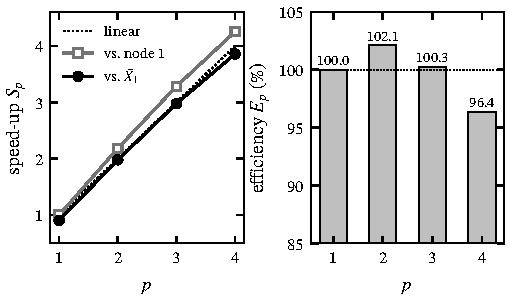
\includegraphics[width=\columnwidth]{fig_speedup.pdf}
\caption{Left: speed-up relative to node N1 and to the mean single node $\bar{X}_1$. Right: efficiency $E_p$ as defined in~\eqref{eq:eff}.}
\label{fig:speedup}
\end{figure}

\subsection{Per-node behaviour and load balance}\label{sec:pernode}
Fig.~\ref{fig:pernode} and Table~\ref{tab:pernode} compare each node's rate alone with its rate while computing inside the four-node run, using the per-chunk compute times reported by the workers. Nodes N2--N4 kept their stand-alone rates to within 1\%. N1 computed 3.7\% faster inside the cluster than in its stand-alone runs, which supports the view that those stand-alone runs were depressed by background load (Section~\ref{sec:anomaly}). The the numbers were divided almost evenly (23.9--25.7\%) although no node was given a fixed share. N1 received the smallest share, consistent with its lower speed. "Busy" is the sum of a node's chunk compute times divided by the job's elapsed time; it was 95.7--98.5\%, so less than 5\% of the time was spent waiting for work.

\begin{table}[t]
\caption{Per-node behaviour in the four-node run}
\label{tab:pernode}
\centering
\begin{tabular}{@{}lrrrr@{}}
\toprule
Node & Alone (MH/s) & In cluster (MH/s) & Share (\%) & Busy (\%) \\
\midrule
N1 & 20.55 & 21.31 & 23.9 & 98.5 \\
N2 & 23.38 & 23.23 & 25.7 & 97.1 \\
N3 & 23.37 & 23.12 & 25.2 & 95.8 \\
N4 & 23.35 & 23.15 & 25.2 & 95.7 \\
\bottomrule
\end{tabular}
\end{table}

\begin{figure}[t]
\centering
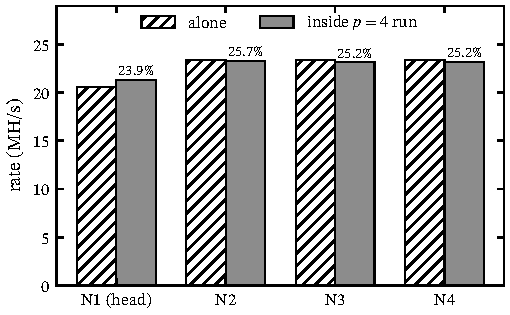
\includegraphics[width=\columnwidth]{fig_pernode.pdf}
\caption{Each node's hashing rate alone and while part of the four-node run. Labels give the node's share of the numbers hashed.}
\label{fig:pernode}
\end{figure}

\subsection{Variability and correctness}
Fig.~\ref{fig:variability} shows the spread of the repeats. Nodes N2--N4 alone varied by less than 1\% (CV), the clusters by 1.4--2.8\%, and N1 alone by 4.8\%. Every repeat of a configuration returned the same number of matching digests (Table~\ref{tab:configs}). The expected count is $n/16^6$, i.e.\ 4.1, 7.7, 11.9 and 16.1 for 70, 130, 200 and 270 million numbers; the observed counts are consistent with these under Poisson variation. This confirms that the distributed runs covered the same input ranges as intended, although it is a consistency check rather than verification against an independent implementation.

\begin{figure}[t]
\centering
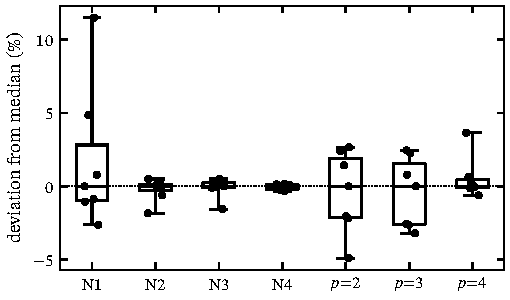
\includegraphics[width=\columnwidth]{fig_variability.pdf}
\caption{Run-to-run variability: deviation of each repeat from its configuration's median (box: quartiles, whiskers: range, dots: individual repeats).}
\label{fig:variability}
\end{figure}

\subsection{Hypothesis tests}
Table~\ref{tab:tests} shows that each added node increased throughput, and that four nodes outperform the fastest single node. All four tests reached the smallest attainable $p$-value, meaning every repeat of the larger configuration was faster than every repeat of the smaller one. The results remain significant at $\alpha = 0.01$ after Bonferroni correction for four tests.

\begin{table}[t]
\caption{One-sided exact permutation tests (7 vs.\ 7 repeats)}
\label{tab:tests}
\centering
\begin{tabular}{@{}lrr@{}}
\toprule
Alternative hypothesis & Gain & $p$ \\
\midrule
$X_2 > X^{(1)}_1$ (N1 alone) & 2.18$\times$ & 0.0003 \\
$X_3 > X_2$ & 1.50$\times$ & 0.0003 \\
$X_4 > X_3$ & 1.29$\times$ & 0.0003 \\
$X_4 > X^{(2)}_1$ (fastest single node) & 3.74$\times$ & 0.0003 \\
\bottomrule
\end{tabular}
\end{table}

\subsection{Live operation}
Fig.~\ref{fig:live} shows the cluster during a run of the project's original example program, \texttt{simple\_sha256.py}, submitted from N1 with \texttt{kit py run examples/simple\_sha256.py --cluster --n 5e7}. The program reports that it ran on the cluster through the Rust engine with four workers and finished in \SI{3.87}{s}. In this mode each chunk is processed by a Python script, so per-node rates (3.4--4.5\,M numbers/s) are much lower than those of the built-in SHA-256 routine used in Table~\ref{tab:configs}. The head's dashboard lists all four nodes at 95--99\% CPU utilisation, and its task stream shows chunks finishing on every node at the same time. These photographs illustrate operation only; all quantitative results above come from the controlled benchmark.

\begin{figure*}[t]
\centering
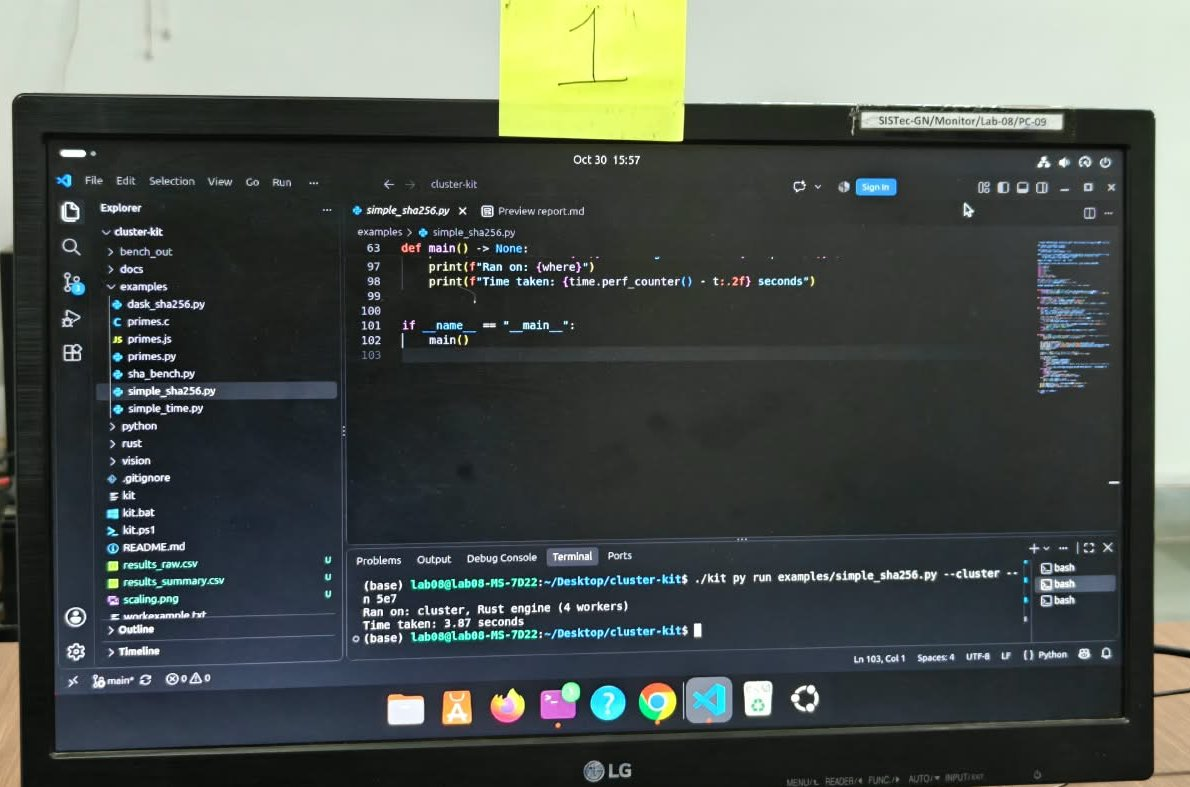
\includegraphics[height=5.2cm]{img/terminal.jpg}\hfill
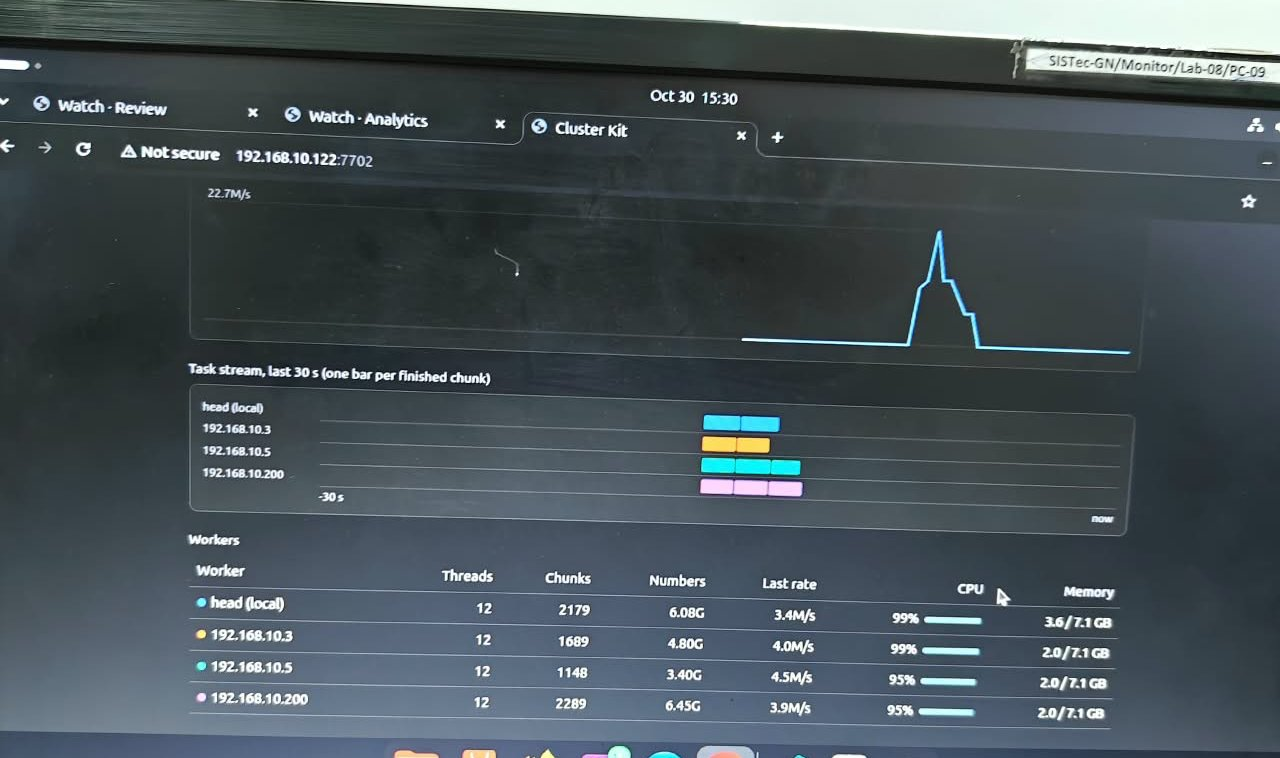
\includegraphics[height=5.2cm]{img/dashboard.jpg}
\caption{Live operation on the testbed. Left: the head node after running \texttt{simple\_sha256.py} on the cluster (``Ran on: cluster, Rust engine (4 workers)''). Right: the head's live dashboard (port 7702), with the per-chunk task stream and all four workers at 95--99\% CPU utilisation.}
\label{fig:live}
\end{figure*}

\section{Discussion}\label{sec:discussion}

\subsection{Why the scaling is near-linear}
The workload has no communication between tasks, and each chunk's input (two integers) and output (a count) are tiny compared with its compute time. Pull-based scheduling adapts to node speed without configuration, and the two-chunk pipeline keeps workers supplied while results travel back. The remaining losses (about 3.6\% at $p = 4$) are consistent with job start-up and the uneven finish of the last chunks, which have a larger relative cost in a run of only about \SI{3}{s}; longer jobs should therefore scale at least as well.

\subsection{The head-node anomaly}\label{sec:anomaly}
Node N1 was 12.1\% slower alone than the mean of the identical N2--N4 (\SI{20.55}{} vs.\ \SI{23.37}{\MHs}) and was the least stable configuration. The most plausible explanation is background load: N1 was the head and was also hosting the project's video-analytics service during the session. This was not isolated experimentally. Because of it, speed-ups relative to N1 (4.25 at $p = 4$) overstate the benefit of clustering, and we treat $S_p$ relative to $\bar{X}_1$ and the heterogeneity-aware $E_p$ as the primary results.

\subsection{Correction of an earlier informal comparison}\label{sec:informal}
An earlier project report compared a single Windows PC (\SI{36.98}{s}) with a four-worker cluster (\SI{2.165}{s}) on a run that found 766 matches, and reported a ratio of 17.08. That ratio is not a valid speed-up. The two sides used different hardware and operating systems and likely different engines (the Python/Dask path is much slower per hash than the Rust engine), and each figure came from a single run. For an embarrassingly parallel workload on four comparable nodes, the scaled speed-up cannot exceed roughly four, which agrees with the 3.86 measured here under controlled conditions.

\subsection{Comparison with MPI}\label{sec:mpi}
MPI~\cite{mpi} is the dominant programming model on production supercomputers, so it is the natural reference point. Table~\ref{tab:mpi} contrasts the two designs. The comparison concerns deployment and robustness, not speed: we did not run an MPI implementation of the workload, so we make no claim that Cluster Kit is faster. For a compute-bound workload such as this one, little room for improvement remains, since Cluster Kit already reaches 96.4\% of the nodes' combined stand-alone throughput; a well-written MPI program would be expected to perform similarly. Cluster Kit's advantages lie elsewhere. Zero-configuration discovery removes host lists and remote-shell set-up. Pull-based scheduling absorbs differences in node speed, which matters on a heterogeneous lab floor. Re-queuing lets a job survive the loss of a node, whereas the default MPI error handler aborts the whole job. These properties trade some generality for ease of use: MPI supports arbitrary communication patterns between processes, while Cluster Kit is limited to independent tasks. A measured MPI baseline on the same testbed is planned as future work.

\begin{table}[t]
\caption{Design comparison with typical MPI deployments}
\label{tab:mpi}
\centering\footnotesize
\setlength{\tabcolsep}{3pt}
\begin{tabular}{@{}>{\raggedright\arraybackslash}p{0.22\columnwidth}>{\raggedright\arraybackslash}p{0.36\columnwidth}>{\raggedright\arraybackslash}p{0.36\columnwidth}@{}}
\toprule
Aspect & Typical MPI & Cluster Kit \\
\midrule
Finding nodes & host file written by hand & UDP broadcast, automatic \\
Launching & \texttt{mpirun} over SSH, keys on every node & one command per node \\
Work division & usually static by rank & dynamic, pulled on demand \\
Uneven nodes & slowest rank sets pace & faster nodes take more chunks \\
Node failure & job aborts by default & lost chunks re-queued \\
Communication & any pattern, collectives & master--worker only \\
Mixed OS & same MPI on all nodes & one portable binary \\
\bottomrule
\end{tabular}
\end{table}

\subsection{Practical implications}
At the measured rates, hashing $10^{11}$ numbers would take 81\,min on N1 and 19\,min on four nodes. For the search problem itself, each additional zero digit multiplies the expected work by 16 (Table~\ref{tab:kzeros}). A four-fold speed-up extends the feasible difficulty by only $\log_{16} 4 = 0.5$ digits, which illustrates why production proof-of-work systems use specialised hardware rather than general-purpose clusters.

\begin{table}[t]
\caption{Expected time to find one digest with $k$ leading zero hex digits ($16^k$ hashes)}
\label{tab:kzeros}
\centering
\begin{tabular}{@{}crrr@{}}
\toprule
$k$ & Expected hashes & N1 alone & 4 nodes \\
\midrule
6 & \num{1.68e7} & 0.82\,s & 0.19\,s \\
8 & \num{4.29e9} & 3.5\,min & 49\,s \\
10 & \num{1.10e12} & 14.9\,h & 3.5\,h \\
12 & \num{2.81e14} & 158.5\,d & 37.3\,d \\
\bottomrule
\end{tabular}
\end{table}

\subsection{Threats to validity}
\emph{Internal validity.} The background load on N1 was not controlled; the interleaved run order reduces but does not remove the effect of slow drift. Runs were short (about \SI{3}{s}), so start-up costs are a larger fraction than in long jobs. \emph{Construct validity.} Throughput was timed by the client and includes job submission and result collection, which is the user-visible time but mixes computation and coordination. Per-node "busy" values are derived from worker-reported compute times, not from operating-system counters. \emph{External validity.} SHA-256 search is close to the best case for distributed computing. Workloads with large inputs, shared state or frequent communication will scale less well, and results on Wi-Fi or a congested network may differ. All measurements come from one session on one LAN.

\section{Conclusion and Future Work}
On four identical commodity workstations, Cluster Kit achieved a speed-up of 3.86 over the mean single node at 96.4\% parallel efficiency on a SHA-256 search workload, with every added node giving a statistically significant improvement, an even work split without manual tuning, and identical results across repeats. Simple design choices (self-scheduling, pipelined chunks and a compact binary protocol) were enough to reach near-linear scaling for independent tasks. Future work includes strong-scaling experiments with a fixed problem size and longer runs, isolating the head-node overhead by running the head on a dedicated machine, evaluating workloads with substantial data movement, measuring GPU-equipped workers, and scaling beyond four nodes to locate the point at which the single head becomes a bottleneck.

\begin{thebibliography}{99}
\bibitem{amdahl} G.~M. Amdahl, ``Validity of the single processor approach to achieving large scale computing capabilities,'' in \emph{Proc. AFIPS Spring Joint Computer Conf.}, 1967, pp.~483--485.
\bibitem{gustafson} J.~L. Gustafson, ``Reevaluating Amdahl's law,'' \emph{Commun. ACM}, vol.~31, no.~5, pp.~532--533, 1988.
\bibitem{karpflatt} A.~H. Karp and H.~P. Flatt, ``Measuring parallel processor performance,'' \emph{Commun. ACM}, vol.~33, no.~5, pp.~539--543, 1990.
\bibitem{beowulf} T.~Sterling, D.~J. Becker, D.~Savarese, J.~E. Dorband, U.~A. Ranawake, and C.~V. Packer, ``Beowulf: A parallel workstation for scientific computation,'' in \emph{Proc. Int. Conf. Parallel Processing (ICPP)}, 1995.
\bibitem{hoefler} T.~Hoefler and R.~Belli, ``Scientific benchmarking of parallel computing systems: Twelve ways to tell the masses when reporting performance results,'' in \emph{Proc. Int. Conf. High Performance Computing, Networking, Storage and Analysis (SC15)}, 2015.
\bibitem{mpi} Message Passing Interface Forum, \emph{MPI: A Message-Passing Interface Standard, Version 4.0}, 2021.
\bibitem{mapreduce} J.~Dean and S.~Ghemawat, ``MapReduce: Simplified data processing on large clusters,'' in \emph{Proc. 6th USENIX Symp. Operating Systems Design and Implementation (OSDI)}, 2004.
\bibitem{dask} M.~Rocklin, ``Dask: Parallel computation with blocked algorithms and task scheduling,'' in \emph{Proc. 14th Python in Science Conf. (SciPy)}, 2015, pp.~130--136.
\bibitem{boinc} D.~P. Anderson, ``BOINC: A system for public-resource computing and storage,'' in \emph{Proc. 5th IEEE/ACM Int. Workshop on Grid Computing}, 2004, pp.~4--10.
\bibitem{factoring} S.~F. Hummel, E.~Schonberg, and L.~E. Flynn, ``Factoring: A method for scheduling parallel loops,'' \emph{Commun. ACM}, vol.~35, no.~8, pp.~90--101, 1992.
\bibitem{fips180} National Institute of Standards and Technology, ``Secure Hash Standard (SHS),'' FIPS PUB 180-4, 2015.
\bibitem{bitcoin} S.~Nakamoto, ``Bitcoin: A peer-to-peer electronic cash system,'' 2008. [Online]. Available: https://bitcoin.org/bitcoin.pdf
\bibitem{rayon} Rayon contributors, ``Rayon: A data parallelism library for Rust.'' [Online]. Available: https://github.com/rayon-rs/rayon
\bibitem{bootstrap} B.~Efron and R.~J. Tibshirani, \emph{An Introduction to the Bootstrap}. New York: Chapman \& Hall, 1993.
\bibitem{permutation} P.~Good, \emph{Permutation, Parametric, and Bootstrap Tests of Hypotheses}, 3rd~ed. New York: Springer, 2005.
\end{thebibliography}

\appendix[Raw measurements]
Table~\ref{tab:raw} lists all 49 timed runs (benchmark identifier \texttt{20261030-150048-cpu}) in the order they were executed.

\begin{table}[h]
\caption{All timed runs}
\label{tab:raw}
\centering\footnotesize
\setlength{\tabcolsep}{3.5pt}
\begin{tabular}{@{}lrrrrr@{}}
\toprule
Config. & Rep. & $n$ & Time (s) & MH/s & Matches \\
\midrule
N1 & 1 & 68,000,000 & 2.968 & 22.91 & 5 \\
N2 & 1 & 70,000,000 & 2.994 & 23.38 & 5 \\
N3 & 1 & 70,000,000 & 3.042 & 23.01 & 5 \\
N4 & 1 & 70,000,000 & 2.994 & 23.38 & 5 \\
$p{=}2$ & 1 & 130,000,000 & 2.898 & 44.86 & 8 \\
$p{=}3$ & 1 & 200,000,000 & 3.042 & 65.75 & 16 \\
$p{=}4$ & 1 & 270,000,000 & 3.090 & 87.38 & 21 \\
N1 & 2 & 68,000,000 & 3.156 & 21.55 & 5 \\
N2 & 2 & 70,000,000 & 2.992 & 23.40 & 5 \\
N3 & 2 & 70,000,000 & 2.989 & 23.42 & 5 \\
N4 & 2 & 70,000,000 & 2.993 & 23.39 & 5 \\
$p{=}2$ & 2 & 130,000,000 & 2.962 & 43.89 & 8 \\
$p{=}3$ & 2 & 200,000,000 & 3.044 & 65.70 & 16 \\
$p{=}4$ & 2 & 270,000,000 & 3.094 & 87.27 & 21 \\
N1 & 3 & 68,000,000 & 3.344 & 20.33 & 5 \\
N2 & 3 & 70,000,000 & 3.012 & 23.24 & 5 \\
N3 & 3 & 70,000,000 & 2.995 & 23.37 & 5 \\
N4 & 3 & 70,000,000 & 3.008 & 23.27 & 5 \\
$p{=}2$ & 3 & 130,000,000 & 3.047 & 42.66 & 8 \\
$p{=}3$ & 3 & 200,000,000 & 3.062 & 65.32 & 16 \\
$p{=}4$ & 3 & 270,000,000 & 3.082 & 87.61 & 21 \\
N1 & 4 & 68,000,000 & 3.309 & 20.55 & 5 \\
N2 & 4 & 70,000,000 & 2.988 & 23.43 & 5 \\
N3 & 4 & 70,000,000 & 2.980 & 23.49 & 5 \\
N4 & 4 & 70,000,000 & 2.998 & 23.35 & 5 \\
$p{=}2$ & 4 & 130,000,000 & 2.857 & 45.50 & 8 \\
$p{=}3$ & 4 & 200,000,000 & 2.964 & 67.48 & 16 \\
$p{=}4$ & 4 & 270,000,000 & 3.109 & 86.84 & 21 \\
N1 & 5 & 68,000,000 & 3.283 & 20.71 & 5 \\
N2 & 5 & 70,000,000 & 3.050 & 22.95 & 5 \\
N3 & 5 & 70,000,000 & 2.996 & 23.36 & 5 \\
N4 & 5 & 70,000,000 & 3.006 & 23.29 & 5 \\
$p{=}2$ & 5 & 130,000,000 & 2.830 & 45.94 & 8 \\
$p{=}3$ & 5 & 200,000,000 & 2.941 & 68.00 & 16 \\
$p{=}4$ & 5 & 270,000,000 & 3.070 & 87.95 & 21 \\
N1 & 6 & 68,000,000 & 3.398 & 20.01 & 5 \\
N2 & 6 & 70,000,000 & 2.994 & 23.38 & 5 \\
N3 & 6 & 70,000,000 & 2.987 & 23.43 & 5 \\
N4 & 6 & 70,000,000 & 3.001 & 23.33 & 5 \\
$p{=}2$ & 6 & 130,000,000 & 2.823 & 46.05 & 8 \\
$p{=}3$ & 6 & 200,000,000 & 2.898 & 69.01 & 16 \\
$p{=}4$ & 6 & 270,000,000 & 3.091 & 87.35 & 21 \\
N1 & 7 & 68,000,000 & 3.338 & 20.37 & 5 \\
N2 & 7 & 70,000,000 & 2.979 & 23.50 & 5 \\
N3 & 7 & 70,000,000 & 2.998 & 23.35 & 5 \\
N4 & 7 & 70,000,000 & 2.995 & 23.37 & 5 \\
$p{=}2$ & 7 & 130,000,000 & 2.958 & 43.95 & 8 \\
$p{=}3$ & 7 & 200,000,000 & 2.893 & 69.13 & 16 \\
$p{=}4$ & 7 & 270,000,000 & 2.981 & 90.57 & 21 \\
\bottomrule
\end{tabular}
\end{table}

\end{document}
